\makeatletter\def\input@path{{styles/}{corps/}{imgs/}{bib/}}\makeatother

% compiler avec: pdflatex rapport && biber rapport && pdflatex rapport

% Utiliser le style guide.cls
\documentclass{guide}


\title{Projet Sécurité des systèmes \\ Cryptograhie légère}
\author{Paul Bouquet \\ Cédric Delaunay \\ Alexandre Degurse}
\date{\today}
\doctype{Rapport}
\promo{CI2019}
\etablissement{\textsc{Ensta} Bretagne\\2, rue Francois Verny\\
  29806 \textsc{Brest} cedex\\\textsc{France}\\Tel +33 (0)2 98 34 88 00\\ \url{www.ensta-bretagne.fr}}
\logoEcole{\includegraphics[height=4.2cm]{logo_ENSTA_Bretagne_Vertical_CMJN}}


\usepackage{xcolor}
\usepackage{fancyhdr}
\usepackage{lastpage}
\usepackage{calc}
\usepackage{graphicx}
\usepackage{subfig}
\usepackage{wrapfig}
\usepackage{caption}
\usepackage{float}
\usepackage[backend=biber,sorting=none]{biblatex}

\usepackage{array}
\usepackage{amssymb}
\usepackage{amsmath}

% Pour écrire du pseudo code
\usepackage{algorithm}
\usepackage{algorithmic}

\newcommand*\xor{\mathbin{\oplus}}

\addbibresource{bib/biblatex.bib}

\footskip=70pt
\def\companylogo{\includegraphics[scale=0.2]{imgs/ensta.jpg}}
\fancypagestyle{companypagestyle}{
    \fancyhf{}
    \fancyfoot[C]{\textbf{Page \thepage/ \pageref{LastPage}}}
    \fancyfoot[R]{
    \parbox[b]{\dimexpr\linewidth-2.5cm\relax}{\sffamily \bfseries\hfill \      {\color{black}\rule{\dimexpr\linewidth\relax}{0.4pt}}\        				{\color{white}sat}
    } }
    \fancyfoot[L]{
    \parbox[b]{2cm}{\companylogo}%
    }
    }

\pagestyle{companypagestyle}

\captionsetup[subfigure]{labelformat=empty}

% creer le glossaire
\makeglossaries
% creer l'index
\makeindex

\begin{document}

  % Début du préambule
  \frontmatter

  \maketitle

  
\section*{Résumé}

  

% \section*{Mots clés}
%
%
%
%
% \selectlanguage{english}
% \section*{Abstract}
%
%
%
% \selectlanguage{french}


  \clearpage

  % table des matieres

  \tableofcontents

  \clearpage


  % Partie principale
  \mainmatter
  % chargement du fichier corps.tex
  \newpage
\part{Introduction à la cryptographie légère}

		L'objectif de ce projet est d'expliquer le fonctionnement des algorithmes de crypto légère (lightweight cryptography).
	Il est demandé de choisir deux algorithmes de cryptographie légère, de les expliquer,
	de les implémenter et de donner des valeurs de performance aussi bien pour des solutions académiques qu'industrielles.
	Il est également demandé de détailler les domaines d'utilisation de ce type d'algorithme.

	\section{Généralités}

			La cryptographie légère est une branche de la cryptographie apparue assez
		récemment, et s’étant peu à peu démocratisée au cours de ces vingt
		dernières années. Sa création est née d’un besoin de sécuriser des
		appareils informatiques de plus en plus petits et de plus en plus
		nombreux. Aujourd’hui, en 2018, on peut dénombrer  plus de  quinze
		milliards d’objets connectés \cite{renaud_developpement_2017}, et ces
		produits nécessitent d’être sécurisés. Si les ordinateurs et mêmes les
		smartphones de dernière génération offrent une puissance de calcul
		permettant d’implémenter facilement les algorithmes de cryptographie
		standard, comme par exemple celui du standard AES (algorithme Rinjdael
		\cite{AES-FIPS}) ou encore RSA, ce n’est pas le cas pour les objets les
		moins puissants et les plus petits comme par exemple les puces RFID,
		certains systèmes embarqués ou les réseaux de capteurs (aussi connus sous
		leur nom anglais « Sensors Networks ») \cite{Report_light}. Cette
		impossibilité d’utiliser des standards de chiffrement « lourds » provient
		en effet d’un manque de puissance de calcul mais aussi dans la plupart de
		cas d’un manque d’espace, aussi bien physique que mémoire.

			On comprend alors l’objet et les enjeux de la cryptographie légère :
		sécuriser, au moyen d’algorithmes moins coûteux, que ce soit en termes de
		temps d’exécution ou d’espace mémoire, l’ensemble des systèmes informatiques
		actuels qui ne peuvent être couverts par les standards de la cryptographie «
		traditionnelle ».

	\section{Les différences entre cryptographie « traditionnelle » et cryptographie légèrele}

			Avant de commencer la présentation des algorithmes de cryptographie légère que
		nous avons choisi d’implémenter, nous pensons qu’il est de bon ton de décrire
		les éléments qui permettent de différencier cryptographie légère et «
		traditionnelle ».

			Commençons par les algorithmes de chiffrement par bloc, dont AES fait partie,
		au même titre que PRESENT qui sera évoqué dans la partie 2 mais qui lui fait
		partie des algorithmes de cryptographie légère. Ces derniers se démarquent des
		algorithmes de cryptographie standard d’abord par des tailles de bloc plus
		petites. Là où AES utilise des blocs de 128 bits \cite{AES-FIPS}, le
		chiffrement par blocs en cryptographie légère fait le plus souvent appel à des
		blocs de 64 ou 80 bits \cite{Report_light}. De même, les clés utilisées sont
		elles aussi plus courtes : 128, 192 ou 256 bits pour AES \cite{AES-FIPS}
		tandis que l’algorithme PRESENT par exemple utilise des clés de 80 bits
		\cite{PRESENT}. De plus, les rondes de ces algorithmes sont simplifiées, avec
		notamment des « S-Box » de quatre bits au lieu de huit dans la plupart des
		algorithmes légers. Cela se traduit notamment par un espace physique requis
		plus faible. En effet, la S-Box de l’AES nécessite 395 GE \cite{RFID} (« gate
		equivalents ») alors que la S-Box utilisée par PRESENT n’en nécessite que 28.
		Pour rappel, le « gate equivalent » est une unité de mesure utilisée en
		électronique qui permet de spécifier la complexité des circuits électroniques
		en indiquant un nombre de portes logiques nécessaires à la réalisation d’une
		fonction. Le constructeur pourra alors avec ce GE savoir l’espace physique
		nécessaire pour réaliser ladite fonction \cite{wiki_gate}. Pour vous donner
		une idée plus précise des ordres de grandeur mis en jeu, on peut noter qu’une
		puce RFID possède une surface généralement comprise entre 1000 et 10000 GE, et
		seulement 200 à 2000 sont dédiées à la sécurité \cite{Report_light}. Enfin,
		les algorithmes de chiffrement par blocs en cryptographie légère implémentes
		des opérations sur les clés de chiffrement beaucoup plus simples et beaucoup
		moins coûteux qu’en cryptographie standard.

			D’autre part, intéressons-nous cette fois aux algorithmes de hachage. Tout
		d’abord, la principale différence réside dans la taille des états internes et
		des hachés produits par l’algorithme. Par exemple, SHA-2 sort des hachés de
		256 bits tandis que SPONGENT (algorithme présenté dans la deuxième partie)
		retourne des hachés qui peuvent descendre jusqu’à 88 bits \cite{6275435}. De
		plus, une autre différence entre ces algorithmes de hachage se situe dans la
		taille des messages en entrée des algorithmes. Là où des algorithmes standards
		peuvent travailler sur des messages très grands (264 bits), les algorithmes de
		hachage de cryptographie légère travaillent sur des données d’entrée beaucoup
		plus faibles, plutôt de l’ordre de $2^8$ bits.

			Enfin, il faut tout de même noter que la cryptographie légère n’a pas que des
		avantages face à la cryptographie traditionnelle. En effet, réduire les
		tailles des blocs, des clés, a un coût en termes de sécurité. Par exemple,
		l’utilisation de blocs de 64 bits dans certains algorithmes réduit
		considérablement le nombre de sorties possibles d’un algorithme, et dans ces
		cas-là un chiffré peut-être différencié d’une séquence aléatoire en utilisant
		seulement 232 blocs. Il en résulte alors que certains algorithmes sont
		vulnérables aux attaques de type « plaintext recovery » ou « key recovery »
		avec des probabilités non négligeables.

\part{Présentation de deux algorithmes de cryptographie légère}

	\section{SPONGENT}

			Cette partie a pour objectif de présenter l’algorithme de cryptographie légère
		SPONGENT. Il découle directement de l’algorithme PRESENT, développé en 2007
		par « Orange Labs », la « Ruhr University Bochum » et la « Technical
		University of Denmark ». Ce dernier est un algorithme par blocs (de 64 bits)
		dont la clé fait 80 ou 128 bits \cite{PRESENT}, et il a la particularité
		d’avoir été inclus au dernier standard international des méthodes de
		cryptographie légère par l’ « International Electrotechnical Commission »
		\cite{ultraLightURL}.

		\subsection{Fonctionnement général de SPONGENT}

			\begin{figure}[!h]
				 	\centering
				 	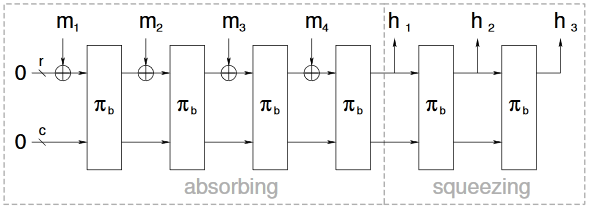
\includegraphics[width=0.9\textwidth]{imgs/Spongent/fctGlobalSpongent.png}
				 	\caption{Schéma illustrant le fonctionnement de SPONGENT, tiré de \cite{6275435}}
				 	\label{fctGlobalSpongent}
			\end{figure}

				Comme énoncé précédemment, SPONGENT s’appuie sur le fonctionnement de
			l’algorithme PRESENT. Pour un nombre fini de bits en entrée, SPONGENT va
			produire un hach de taille n (fixé). La figure \ref{fctGlobalSpongent}
			schématise le fonctionnement de l’algorithme, qui s’organise en trois
			phases distinctes, que sont l’initialisation, l’absorption (absorbing) et
			le relâchement (squeezing).

			 	L’initialisation consiste à ajouter un 1 binaire suivi de x 0 afin que la
			taille du message en entrée soit un multiple de la taille des blocs, appelé
			r (rate en anglais). Le message est ensuite découpé en blocs de r bits.
			Ensuite vient la phase d’absorption. Durant cette phase, un bloc $m_{i}$
			subit un XOR avec les r premiers bits de l’état courant et passe ensuite
			dans la fonction de permutation. Cette permutation génère un état de b
			bits, où $b = r + c$, et où c est appelé la capacité de l’état et b est
			appelé la largeur de l’état. Enfin, la phase de relâchement consiste à
			retourner les r premiers bits de l’état, puis de passer l’état dans la
			fonction de permutation, et de répéter ces deux opérations jusqu’à ce que
			le hach retourné ait une longueur de n bits.

				Les valeurs de n, b, c et r ne sont pas prises au hasard. En effet, il
			existe treize versions différentes de SPONGENT et elles sont définies grâce
			au tableau représenté à la figure \ref{variantesSpongent}. Ces treize
			versions s’appuient sur des hachés de tailles différentes, mais les valeurs
			des trois autres constantes citées ci-avant diffèrent elles-aussi selon la
			version utilisée. Dans le cas de notre projet, nous avons décidé
			d’implémenter SPONGENT 160/160/80.

			\begin{figure}[!h]
				\centering
				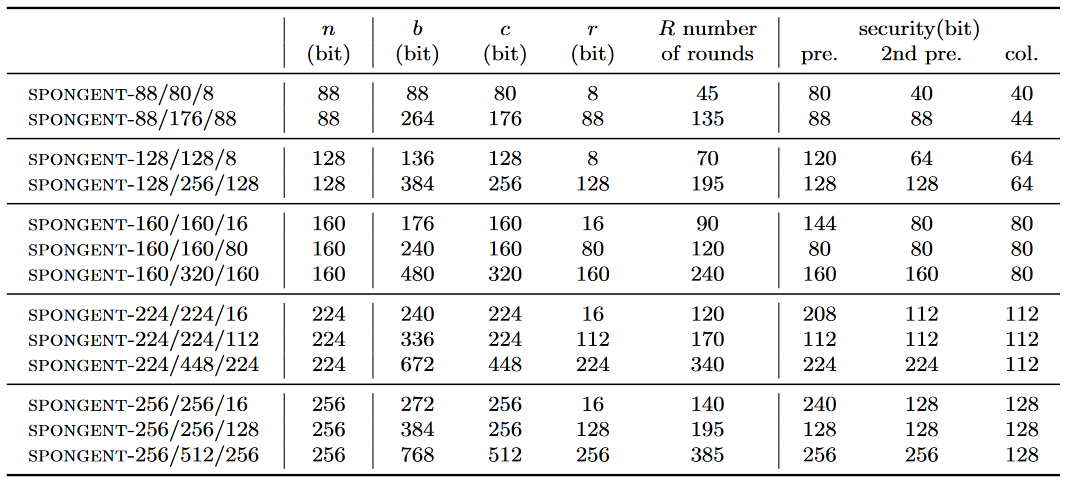
\includegraphics[width=\textwidth]{imgs/Spongent/varianteSpongent.png}
				\caption{Tableau définissant  les 13 variantes de SPONGENT, tiré de \cite{6275435}}
				\label{variantesSpongent}
	 		\end{figure}

		\subsection{Fonctionnement détaillé de SPONGENT 160 / 160 / 80}

				Cette sous-partie va permettre d’expliquer le fonctionnement détaillé de la
			permutation notée $\pi_{b}$. Cette permutation est définie par l’algorithme
			\ref{algoSpongent}:

			\begin{algorithm}
				\caption{Algorithme de permutation de SPONGENT}
				\label{algoSpongent}
				\begin{algorithmic}
					\FOR{i = 1 to R}
						\STATE $ STATE \leftarrow $ \reflectbox{$lCounter_{b}$}$(i) \xor STATE \xor lCounter_{b}(i)$
						\STATE $ STATE \leftarrow sBoxLayer_{b}(STATE)$
						\STATE $ STATE \leftarrow pLayer_{b}(STATE)$
					\ENDFOR
				\end{algorithmic}
			\end{algorithm}

				Tout d’abord, intéressons-nous aux variables de cet algorithme. La
			variable R est le nombre de rondes de l’algorithme. Il varie en fonction
			de la variante de SPONGENT utilisée, et dans notre cas R vaut 80. Ensuite,
			la variable STATE représente l’état courant.

				La première opération appliquée à STATE est un XOR avec d’une part
			lCounterb(i) et d’autre part la valeur « retournée » de lCounterb(i),
			c’est-à-dire que si lCounterb(i) = 1000 sa valeur « retournée » est 0001.
			lCounterb(i) est en réalité un LFSR, ou Registre à décalage à rétroaction
			linéaire, soit un générateur pseudo-aléatoire qui dépend lui aussi de la
			variante de l’algorithme utilisée. La figure \ref{polyPrimitifsLFSR}
			illustre les polynômes générateurs du LFSR, et la figure \ref{valInitLFSR}
			indique les valeurs initiales que prend le LFSR.

			\begin{figure}[!htb]
				\begin{minipage}{0.48\textwidth}
				  \centering
				  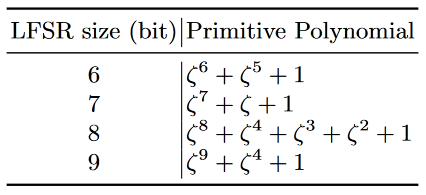
\includegraphics[width=0.9\textwidth]{imgs/Spongent/PrimiPolySpongent.png}
				  \caption{Polynômes primitifs du LFSR}
				  \label{polyPrimitifsLFSR}
				\end{minipage}
				\hfill
				\begin {minipage}{0.48\textwidth}
				  \centering
				  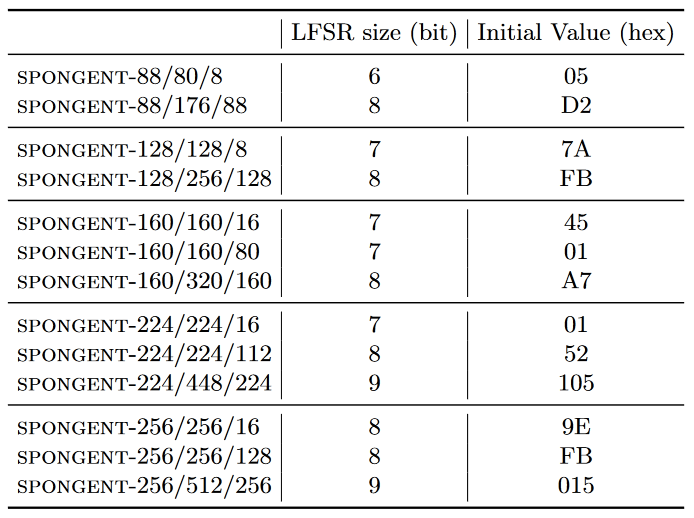
\includegraphics[width=0.9\textwidth]{imgs/Spongent/valInitLFSR.png}
				  \caption{Valeurs initiales du LFSR}
				  \label{valInitLFSR}
				\end{minipage}
			 \end{figure}

				La deuxième opération de la ronde est de passer STATE dans une S-Box.
			La S-Box est la même pour toutes les variantes de l’algorithme SPONGENT
			et elle est définie par la figure \ref{sBoxSpongent.png} :

			\begin{figure}[!h]
				\centering
				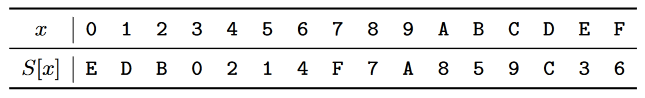
\includegraphics[width=0.9\textwidth]{imgs/Spongent/sBoxSpongent.png}
				\caption{S-Box de l'algorithme SPONGENT}
				\label{sBoxSpongent.png}
			\end{figure}

				Enfin, la troisième et dernière opération est de passer STATE dans $pLayer_{b}$.
			$pLayer_{b}$ est une fonction de permutation définie comme
			l’inverse de la permutation de bits de l’algorithme PRESENT.
			Ainsi, chaque bit j est permuté avec le bit de position $P_{b}(j)$ où :

			\begin{figure}[!htbp]
				\centering
			\begin{equation}
				P_{b}(j) = \begin{cases}
				  j \cdot \frac{b}{4} \bmod b - 1, if j \in \{0, \dots, b - 2\}\\
				  b - 1, if j = b - 1.
				\end{cases}
			  \end{equation}
			  \caption{Formule de permutation de pLayer}
				\label{pLayer}
			\end{figure}

		\subparagraph{Performances et sécurité}

			Les variantes de SPONGENT peuvent être implémentées en utilisant entre 738
		GE (pour SPONGENT 80/80/8) et 5100 GE (pour SPONGENT 256/512/256). Ces
		nombres ne semblent peut-être pas très explicites, mais ils dénotent une
		très grande compacité de l’implémentation physique de l’algorithme. Pour
		plus de détails, la figure \ref{espacePhysique} présente pour différentes
		variantes de l’algorithme l’espace physique nécessaire en fonction de la
		technologie (NXP, UMC et NANGATE)\cite{googleSpongent} :

		\begin{figure}[!h]
			\centering
			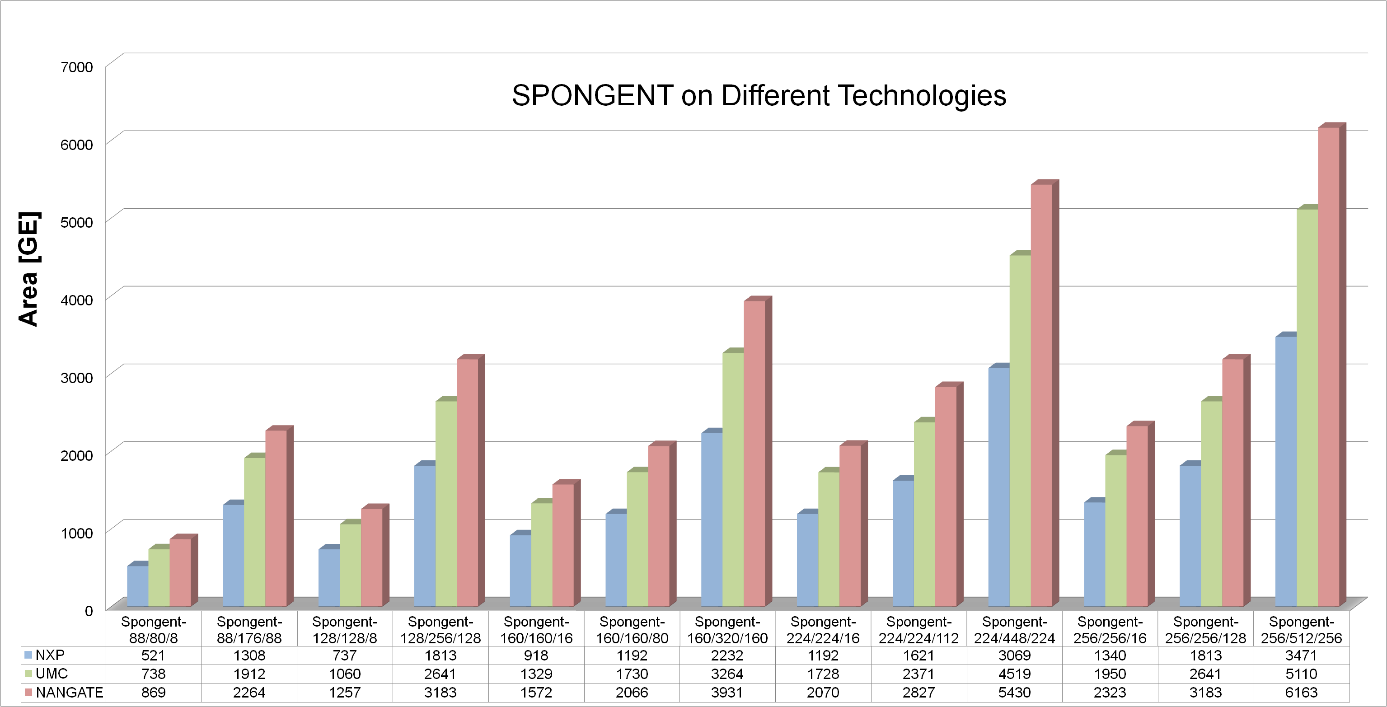
\includegraphics[width=0.9\textwidth]{imgs/Spongent/espacePhysiqueVariante.png}
			\caption{Espace physique nécessaire pour différentes variantes de SPONGENT}
			\label{espacePhysique}
		\end{figure}

			Pour ce qui est du débit de traitement, il est donné comme variant entre 360
		Mbps et 2 Gbps (en fonction de la variante de SPONGENT utilisée). En
		comparaison, l’algorithme de hachage SHA-1 possède un débit de l’ordre d’ 1
		Gbps \cite{SHA1}.

		\begin{figure}[!h]
			\centering
			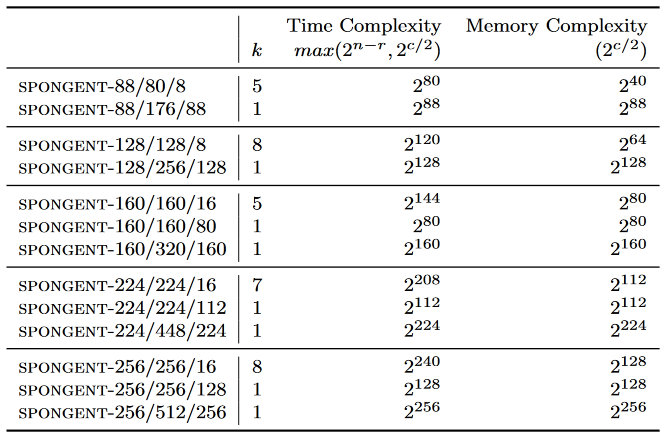
\includegraphics[width=0.9\textwidth]{imgs/Spongent/timeComplexity.png}
			\caption{Complexités en temps et en mémoire de SPONGENT}
			\label{timeComplexity}
		\end{figure}

			En termes de sécurité, nous pouvons voir sur la figure \ref{timeComplexity}
		les différentes valeurs de complexité pour l’ensemble des variantes de
		SPONGENT. Pour les variantes 88/80/8 et 128/128/8, il est intéressant de
		noter que nous sommes dans des capacités de calcul atteignables, et que de
		ce fait ces algorithmes ne sont pas « sûrs ». Pour le reste, nous pouvons
		observer des complexités relatives au minimum inatteignable ($2^{80}$) voire
		raisonnablement inatteignable ($2^{128}$).

			Enfin, la figure \ref{attaquePreImage} présente les résultats de sécurité
		face aux attaques par pré-image, par 2\up{ème} pré-image et par collision
		\cite{googleSpongent}. L’attaque par pré-image consiste, à partir d’un haché
		$y$, à retrouver un $x$ tel que $h(x) = y$. L’attaque par 2\up{ème}
		pré-image consiste quant à elle, à partir d’un clair $x$, à trouver $x’$ tel
		que $h(x) = h(x’)$. Enfin, l’attaque par collision consiste à essayer de
		trouver deux clairs différents produisant le même chiffré. Elle ressemble à
		l’attaque par 2\up{ème} pré-image à ceci près que le clair n’est pas
		spécifié.

		\begin{figure}[!h]
			\centering
			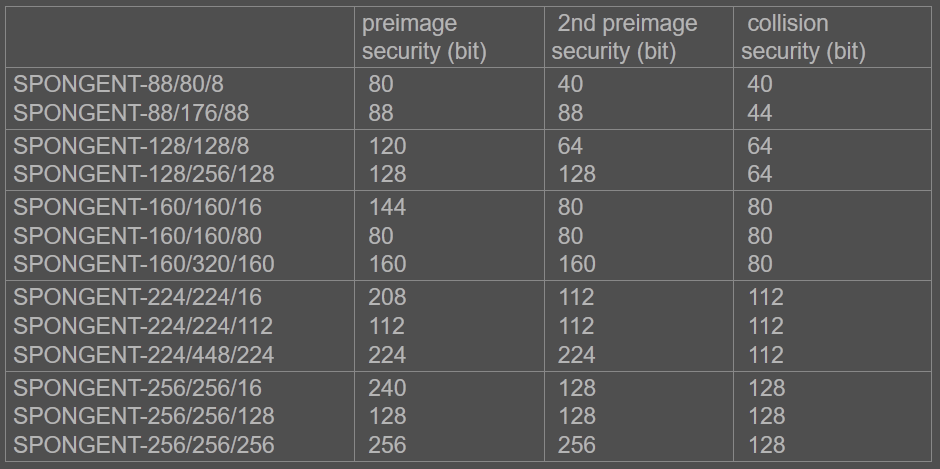
\includegraphics[width=0.9\textwidth, height=0.3\textheight]{imgs/Spongent/attaquePreImage.png}
			\caption{Attaque par pré-image et collision}
			\label{attaquePreImage}
		\end{figure}

		\section{Speck}

			Speck est un algorithme de chiffrement par bloc léger crée par la
		\textit{National Security Agency} (NSA) et rendu
		publique en 2013. C'est un algorithme spécialement conçu pour avoir des performances
		élevées afin d'offrir un algorithme de chiffrement utilisable dans le cadre de
		"l'Internet of Things".

		\subsection{Algorithmes ARX}

				Cet algorithme fait parti des algorithmes dits ARX, Add-Rotate-Xor. C'est une famille
			d'algorithmes qui n'utilisent que les opérations d'additions, rotations et ou exclusif
			dans l'espace $GF_{2^n}$. Il y a plusieurs avantages à se limiter à ces opérations:

			\begin{enumerate}
			\item[•] Rapidité: ces opérations sont des opérations logiques. Ainsi, elles sont
				des primitives de tout micro-controlleur et donc sont effectué en un seul
				cycle d'horloge.
			\item[•] Sécurité matérielle: le fait que toutes les opérations soient des opérations
				logiques atomiques permet à ces algorithmes de fonctionner en temps constant.
				Prévenant les attaques par canaux cachés basés sur les mesures de temps.
			\item[•] Implémentation: ces algorithmes sont souvent très simples. Leur implémentation
				qu'elle soit logicielle ou matérielle est très simple. Par conséquent, le
				temps de développement et le coût de leur implémentation est très faible.
			\end{enumerate}

		\subsection{Fonctionnement de Speck}

			Avant de détailler comment fonctionne Speck, considérons les notations suivantes:

			\begin{enumerate}
			  \item[•] Le ou-exclusif bit à bit, noté xor
			  \item[•] L'addiction modulo $2^n$, noté $\xor$
			  \item[•] Les rotations circulaires à gauche et à droite respectivement notées,
			    $S^i$ et $S^{-i}$ pour des rotations de i-bits.
			\end{enumerate}

			Un tour de chiffrement de l'algorithme Speck est définit de la façon suivante. \\
			Pour $k \in GF(2^n)$ une clée, le tour de chiffrement est définit par la fonction suivante:
			\[
			\begin{array}{ccccc}
			R_k & : & GF(2^n) x GF(2^n) & \to & GF(2^n) x GF(2^n) \\
			 & & (x,y) & \mapsto & ((S^{-\alpha}(x) + y) \xor k, S^\beta (y) \xor (S^{-\alpha} + y) \xor k) \\
			\end{array}
			\]

			avec $\alpha$ = 7 et $\beta$ = 2 si n = 16, $\alpha $= 8 et $\beta$ = 3 sinon. \\

			La fonction de déchiffrement est définie par:
			\[
			\begin{array}{ccccc}
			R_k^{-1} & : & GF(2^n) x GF(2^n) & \to & GF(2^n) x GF(2^n) \\
			 & & (x,y) & \mapsto & (S^\alpha ((x \xor k) - S^{-\beta}(x \xor y)), S^{-\beta}(x \xor y)) \\
			\end{array}
			\]

			On peut représenter un tour de Speck de la façon suivante:

			\begin{figure}[!h]
				\centering
				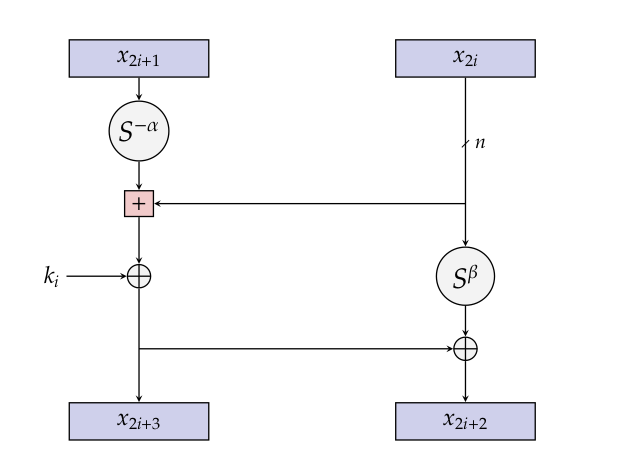
\includegraphics[width=0.9\textwidth]{imgs/roundSpeck.png}
				\caption{i-ème tour de Speck}
			 	\label{roundSpeck}
			\end{figure}

			\vspace{0.3cm}

			Speck pour utiliser un grand nombre de tailles de blocs ainsi que de clées.

			\vspace{0.5cm}

			\begin{figure}[!h]
				\centering
				\begin{tabular}{cc}
					taille de bloc & taille de clée \\
					\hline
					32 & 64 \\
					\hline
					48 & 72,96 \\
					\hline
					64 & 96,128 \\
					\hline
					96 & 96,144 \\
					\hline
					128 & 128,192,256 \\
					\hline
				\end{tabular}
				\caption{Taille de blocs/clées possible pour Speck}
			 	\label{tailleSpeck}
			\end{figure}

			\vspace{0.5cm}

			\part{Domaines d'application}

			\section{Introduction}


			Depuis quelques années, nous pouvons apercevoir un changement dans la puissance des appareils électroniques.
			En effet, on passe d'ordinateur à usage général à des appareils dédiés avec des resources limités.
			Ce changement apporte un large éventail de préoccupations en matière de sécurité et de protection de la vie privée.
			C'est pourquoi il est nécessaire de créer de nouveau standards spécialement adaptés à ces conditions.
			
			Ces nouveaux standards visent essentiellement à utiliser le minimum de GE tout en gardant un niveau de sécurité accceptable pour les applications visées.
			Les questions de consommation de puissance et de rapidité sont aussi à prendre en compte.
			En effet, ces appareils seront destinés à communiquer avec d'autres au sein d'un réseau ou utiliser des batteries.
			
			Il y a déjà plusieurs domaines dans lesquels de tels appareils sont interconnectés and travaillent de concert pour accomplir certaines tâches.
			Comme par exemple : les réseaux de capteurs, les systèmes de contrôles distribués, l'Internet Of Thigs (IoT), le « smart grid », les systèmes embarqués ou encore les dispositifs RFID.
			
			\section{Chiffrement de flux}
			
			Dans cette partie, on s'intéressera uniquement aux aux méthodes de chiffrement de flux.
			Le chiffrement par flot est caractérisé par sa capacité à « chiffrer les caractères (généralement des chiffres binaires) d'un message en clair, un à la fois,
			en utilisant une transformation de chiffrement qui varie avec le temps »\cite{appliedCrypto}.
			
			\begin{figure}[!h]
				\centering
				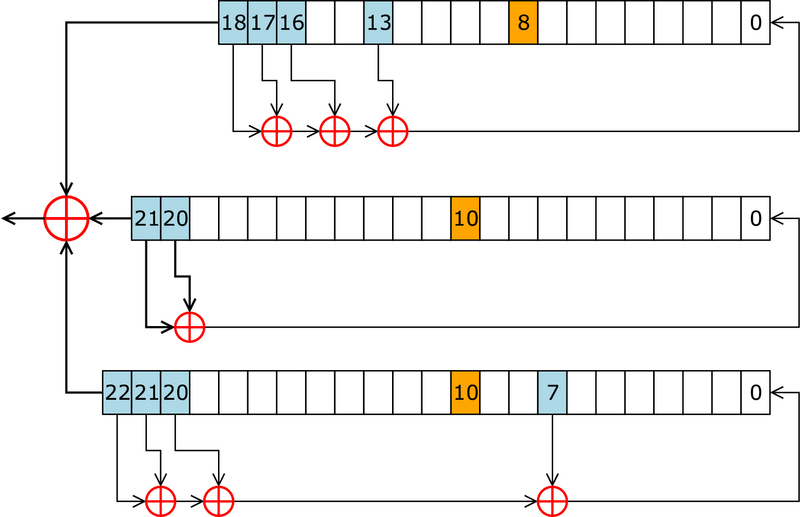
\includegraphics[width=0.9\textwidth]{imgs/application/A5.png}
				\caption{Fonctionnement de l'algorithme A5/1.}
				\label{algoA5}
			\end{figure}
			
			Les méthodes de chiffrement de flux sont naturellment utilisées dans les domaines des télécommunications et de l'audiovisuel.
			Par exemple, les communications qui utilisent le protocole 2G GSM sont chiffrés par l'algorithme A5/1.
			A5/1 est largment utilisé en Europe et aux État-Uni et permet à plus de 7 milliards de téléphone de communiquer de manière sécurisé\cite{7milliards}.
			Les communications de téléphonie par satellite posssèdent souvent aussi leurs algorithme de chiffrement.
			De tels algorithmes sont jalousement gardés par les constructeurs et peu d'entre eux ont été percé à jour, que ce soit avec des attaques classiques ou du « reverse engineering ».
			
			Des algorithmes de chiffrement de flux sont aussi utilisés lors de la lecture de contenu sur certains dvd. Ces dvd sont souvent chiffrés avec l'algorithme Content Scrambling System (Css).
			Ce genre d'algorithme a été développé pour implémenter les Digital Rights Managements (DRM). Ces mesures permettent de protéger à la fois l'accès au contenu mais aussi contre les systèmes de copie.
			
			\subsection{Chiffremment par bloc}
			
			La deuxième grande famille de méthode de chiffrement est le chiffrement par bloc. Il consiste à découper les données à chiffrer en blocs puis de chiffrer ces blocs.
			Le, très connu, AES est un algorithme de chiffrement par bloc.
			
			\begin{figure}[!h]
				\centering
				
\includegraphics[width=0.9\textwidth]{imgs/application/IOT.jpg}
				\label{IOT}
			\end{figure}
			
			Les deux algorithmes présentés dans les parties précédentes sont des méthodes de chiffrement par blocs.
			Speck a été dévloppé, depuis 2012, par la NSA et optimisé pour une utilisation logicielle, tandis que sa contrepartie, Simon, a été optimisé pour une utilisation matérielle.
			De plus, il offre de très bonnes performances même sur des machines à faible puissance de calcul.
			En effet, il peut être implémenté sur des microcontrolleurs de 8 bits.
			Cet algorithme a été développé en vue d'être intégré dans des objets de l'« Internet Of Things ».
			Enfin, Linux a ajouté le support SPECK pour un cryptage efficace et opportuniste sur les périphériques à faibles ressources au noyau en février 2018.
			
			Mais de nombreuses voix s'élèvent contre la NSA et leurs algorithmes, notamment l'ISO (International Organization for Standardization).
			L'organisation internationale n'a pas confiance en la NSA et ses bonnes intentions.
			Saa crédibilité est fortement réduite après l'affaire Snowden et les preuves accusant l'agence de sécurité américaine d'avoir poussé la standardisation d'un algorithme de chiffrement (Dual EC DRBG) qui s'est révélé, plus tard, être « back-doored »\cite{NSABackdoor}.
			
			Un autre algorithme de chiffrement par bloc utilisé de manière commerciale est l'algorithme Cryptomeria, souvent appelé « C2 » dans la littérature.
			Il est utilisé dans les lecteurs de dvd et des cartes SD. Il peut être vu comme le successeur de Css car il vise à remplir la même fonction, c'est-à-dire protéger l'accès au contenu et lutter contre les systèmes de copie.
			
			\section{Conclusion}
			
			Il y a deux grandes familles d'algorithmes de chiffrement : de flux et par bloc.
			On retrouve les deux types d'algorithmes dans des domaines variés comme les télécommunications, l'audiovisuel, \dots
			
			Le chiffrement de flux semble être privilégié car il permettrait de sécuriser la communication des objets interconnectés de l'« Internet Of Things », le défi technologique des décennies à venir.
			Cet attrait est d'autant plus accentué par l'engouement de grandes institutions américaines sur le sujet comme la NSA, avec ses deux algorithmes Speck et Simon, et la NIST (National Institute of Standards and Technology) qui organisent des ateliers sur le sujet.

\newpage
\part*{Conclusion générale}

La cryptographie légère est une branche de la cryptopgraphie apparue récemment et qui s'est développé avec l'apparition de nouveaux appareils éléctroniques de puissances moindres que les ordinateurs classiques.
Commes leurs puissances est plus faibles les algorithmes classiques (RSA, AES) sont trop coûteux pour ces appareils, il a donc fallu passer à des algorithmes plus « léger » et mieux adaptés à ces appareils.
Il faut tout de même noter que ces algorithmes présentent, par design, des faiblesses à certaines attaques.
Deux algorithmes de chiffrement par bloc ont été présentés dans ce rapport : Spongent et Speck.

Spongent s'appuie sur l'algorithme PRESENT qui a été inclus au dernier standard international des méthodes de cryptographie légère par l’ « International Electrotechnical Commission ».
Il en existe treize variantes, dont SPONGENT 160 / 160 / 80 que nous avons implementé en python.
Cet algorithme peut être implementé en utilisant entre 738 et 5100 GE, ce qui montre la compacité physique des implementations.
Les algorithmes de cryptographie légère se démarquent aussi par leurs débits élévés. Pour le SPONGENT, on peut atteindre 2Gps.
En comparaison, SHA-1 a un débit de l'ordre de 1Gps.
En termes de sécurité, pour certaines variantes sont « sûrs » tandis que d'autres ne le sont pas (88/80/8 et 128/128/8).

Le 2\up{ème} algorithme est Speck, développé par la NSA et rendu publique en 2013. Il a été spécialement conçus pour être utilisé dans le cadre de l'« Internet Of Things ».
Tout comme Spongent, Speck peut utiliser une variété de taille de blocs et de clé ce qui le rends très versatile.
% !!! A completer !!

Le développement de la cryptographie légère a suivi la tendance des nouveaux appareils éléctroniques, comme les smartphone ou les tablettes, pour proposer des algorithmes de chiffrement adaptés à ces nouveaux besoins.
Ces nouvelle méthodes de chiffrement peuvent être utilisé dans beaucoup de domaines mais on les retrouve essentiellement dans les télécommunications et l'audiovisuel.
Leurs déveoppements s'accélère avec l'augmentation du nombre des objets interconnectés (« Internet Of Things ») et l'engouement marqué des grandes agences spécialisées dans le domaine comme la NSA et la NIST.

  \nocite{*}

  % Annexes
  \clearpage
  \appendix


  \phantomsection
  \addcontentsline{toc}{section}{Liste des figures}
  \listoffigures

  \phantomsection
  \addcontentsline{toc}{section}{Références}
  \printbibliography



\end{document}